% -*- coding: utf-8 -*-
% Окружение как список записей активаций
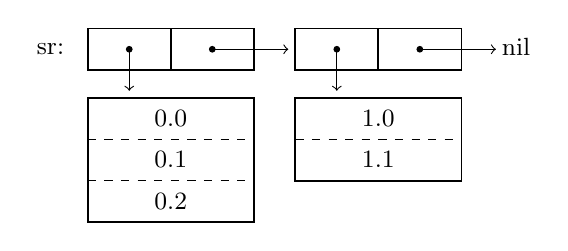
\begin{tikzpicture}
  \tikzstyle{every node}=[font=\small]

% список
  \draw (-0.5em, -0.75em) node[left] {\ic{sr}:};

  \draw [semithick] (0.0em, 0.0em) rectangle (6.0em, -1.5em);
  \draw [semithick] (3.0em, 0.0em) -- (3.0em, -1.5em);

  \filldraw  (4.5em, -0.75em) circle(1.0pt);
  \draw [->] (4.5em, -0.75em) -- (7.25em, -0.75em);

  \draw [semithick] (7.5em, 0.0em) rectangle (13.5em, -1.5em);
  \draw [semithick] (10.5em, 0.0em) -- (10.5em, -1.5em);

  \filldraw  (12.0em, -0.75em) circle(1.0pt);
  \draw [->] (12.0em, -0.75em) -- (14.75em, -0.75em);

  \draw [semithick] (14.6em, -0.65em) node[right] {\ii{nil}};

% окружения
  \filldraw  (1.5em, -0.75em) circle(1.0pt);
  \draw [->] (1.5em, -0.75em) -- (1.5em, -2.25em);
  \draw [semithick] (0.0em, -2.5em) rectangle (6.0em, -7.0em);
  \draw             (3.0em, -2.6em) node[below] {\ic{0.0}};
  \draw [dashed]    (0.0em, -4.0em) -- (6.0em, -4.0em);
  \draw             (3.0em, -4.1em) node[below] {\ic{0.1}};
  \draw [dashed]    (0.0em, -5.5em) -- (6.0em, -5.5em);
  \draw             (3.0em, -5.6em) node[below] {\ic{0.2}};

  \filldraw  (9.0em, -0.75em) circle(1.0pt);
  \draw [->] (9.0em, -0.75em) -- (9.0em, -2.25em);
  \draw [semithick] ( 7.5em, -2.5em) rectangle (13.5em, -5.5em);
  \draw             (10.5em, -2.6em) node[below] {\ic{1.0}};
  \draw [dashed]    ( 7.5em, -4.0em) -- (13.5em, -4.0em);
  \draw             (10.5em, -4.1em) node[below] {\ic{1.1}};

\end{tikzpicture}
